\documentclass[aspectratio=169]{beamer}

\mode<presentation>

\usepackage[utf8]{inputenc}
\usepackage[T1]{fontenc}	%makes å,ä,ö etc. proper symbols
\usepackage{amsmath}
\usepackage{graphicx}
\usepackage{xcolor}
\usepackage{listings}
\usepackage{multicol}
\usepackage{hyperref}


\definecolor{LundaGroen}{RGB}{00,68,71}
\definecolor{StabilaLila}{RGB}{85,19,78}
\definecolor{VarmOrange}{RGB}{237,104,63}

\definecolor{MagnoliaRosa}{RGB}{251,214,209}
\definecolor{LundaHimmel}{RGB}{204,225,225}
\definecolor{LundaLjus}{RGB}{255,242,191}

\usefonttheme{serif}
\usetheme{malmoe}
\setbeamercolor{palette primary}{bg=VarmOrange}
\setbeamercolor{palette quaternary}{bg=LundaGroen}
\setbeamercolor{background canvas}{bg=LundaLjus}
\setbeamercolor{structure}{fg=LundaGroen}

\usepackage[many]{tcolorbox}

\newtcolorbox{cross}{blank,breakable,parbox=false,
  overlay={\draw[red,line width=5pt] (interior.south west)--(interior.north east);
    \draw[red,line width=5pt] (interior.north west)--(interior.south east);}}



\lstset{language=Python} 
\lstset{%language=[LaTeX]Tex,%C++,
    morekeywords={PassOptionsToPackage,selectlanguage,True,False},
    keywordstyle=\color{blue},%\bfseries,
    basicstyle=\small\ttfamily,
    %identifierstyle=\color{NavyBlue},
    commentstyle=\color{red}\ttfamily,
    stringstyle=\color{VarmOrange},
    numbers=left,%
    numberstyle=\scriptsize,%\tiny
    stepnumber=1,
    numbersep=8pt,
    showstringspaces=false,
    breaklines=true,
    %frameround=ftff,
    frame=single,
    belowcaptionskip=.75\baselineskip,
	tabsize=4,
	backgroundcolor=\color{white}
    %frame=L
}

\begin{document}

\lstset{literate=
  {á}{{\'a}}1 {é}{{\'e}}1 {í}{{\'i}}1 {ó}{{\'o}}1 {ú}{{\'u}}1
  {Á}{{\'A}}1 {É}{{\'E}}1 {Í}{{\'I}}1 {Ó}{{\'O}}1 {Ú}{{\'U}}1
  {à}{{\`a}}1 {è}{{\`e}}1 {ì}{{\`i}}1 {ò}{{\`o}}1 {ù}{{\`u}}1
  {À}{{\`A}}1 {È}{{\'E}}1 {Ì}{{\`I}}1 {Ò}{{\`O}}1 {Ù}{{\`U}}1
  {ä}{{\"a}}1 {ë}{{\"e}}1 {ï}{{\"i}}1 {ö}{{\"o}}1 {ü}{{\"u}}1
  {Ä}{{\"A}}1 {Ë}{{\"E}}1 {Ï}{{\"I}}1 {Ö}{{\"O}}1 {Ü}{{\"U}}1
  {â}{{\^a}}1 {ê}{{\^e}}1 {î}{{\^i}}1 {ô}{{\^o}}1 {û}{{\^u}}1
  {Â}{{\^A}}1 {Ê}{{\^E}}1 {Î}{{\^I}}1 {Ô}{{\^O}}1 {Û}{{\^U}}1
  {œ}{{\oe}}1 {Œ}{{\OE}}1 {æ}{{\ae}}1 {Æ}{{\AE}}1 {ß}{{\ss}}1
  {ű}{{\H{u}}}1 {Ű}{{\H{U}}}1 {ő}{{\H{o}}}1 {Ő}{{\H{O}}}1
  {ç}{{\c c}}1 {Ç}{{\c C}}1 {ø}{{\o}}1 {å}{{\r a}}1 {Å}{{\r A}}1
  {€}{{\euro}}1 {£}{{\pounds}}1 {«}{{\guillemotleft}}1
  {»}{{\guillemotright}}1 {ñ}{{\~n}}1 {Ñ}{{\~N}}1 {¿}{{?`}}1
}

% NEW COMMANDS
\newcommand{\fortt}{\texttt{for}}
\newcommand{\whilett}{\texttt{while}}
\newcommand{\iftt}{\texttt{if}}

\AtBeginSection[ ]
{
\begin{frame}{Outline}
    \tableofcontents[currentsection]
\end{frame}
}

\title{GUI 2}
\date{vt 25}
\author{Programmering 2}

\maketitle

\tableofcontents

\section{Repetition}

\subsection{Skapa ett fönster}

\begin{frame}[fragile]
	\frametitle{Repetition}
	\framesubtitle{Skapa ett fönster}
	
	\begin{lstlisting}
import tkinter as tk # tk är standard förkortningen

app = tk.Tk() # Detta skapar själva fönstret

app.mainloop() # Detta ser till att fönstret inte dör
	\end{lstlisting}

\end{frame}

\subsection{Widgets/Element}

\begin{frame}[fragile]
	\frametitle{Repetition}
	\framesubtitle{Våra widgets (element)}
	
	\begin{lstlisting}
def funk():
    ...
	
app = tk.Tk()
tk.Label(app, text="Texten") # Text-widget
tk.Button(app, text="Texten", command=funk) # Knapp-widget
tk.Entry(app) # Ett fält man kan skriva i
	\end{lstlisting}

\end{frame}

\subsection{Placera widgets}

\begin{frame}[fragile]
	\frametitle{Repetition}
	\framesubtitle{Placera element med pack}
	
	\begin{lstlisting}
app = tk.Tk()

min_widget = tk.Label(app, text="Wow")

min_widget.pack() # Placerar ut elementet
	\end{lstlisting}

\end{frame}

\subsection{Get/Set}

\begin{frame}[fragile]
	\frametitle{Repetition}
	\framesubtitle{Get/Set}
	
	\begin{lstlisting}
...
min_widget = tk.Label(app, text="Kolla")

print(min_widget['text']) # Skriver ut kolla
min_widget['text'] = 'Ny text'
print(min_widget['text']) # Skriver ut Ny text
	\end{lstlisting}

\end{frame}

\begin{frame}[fragile]
	\frametitle{Repetition}
	\framesubtitle{Get/Set}
	
	\begin{lstlisting}
mitt_entry = tk.Entry(app)
...
svar = mitt_entry.get()
	\end{lstlisting}

\end{frame}

\section{Placera mera}

\begin{frame}
	\frametitle{Placera mera}
	
	\begin{itemize}
		\item Ibland vill man ha mer koll på sin placering av widgets
		\item Det finns två andra sätt att placera ut widgets på
		\begin{itemize}
			\item \lstinline{grid()}
			\item \lstinline{place()}
		\end{itemize}
	\end{itemize}

\end{frame}

\subsection{Grid}

\begin{frame}[fragile]
	\frametitle{Placera mera}
	\framesubtitle{Grid}
	
	Med \lstinline{grid()} placerar man ut elementen i rader och kolumner.
	
	\begin{lstlisting}
app = tk.Tk()
min_widget1 = tk.Label(app, text="1")
min_widget2 = tk.Label(app, text="2")
min_widget3 = tk.Label(app, text="3")
min_widget4 = tk.Label(app, text="4")

min_widget1.grid(row=0, column=0)
min_widget2.grid(row=0, column=1)
min_widget3.grid(row=1, column=0)
min_widget4.grid(row=1, column=1)
	\end{lstlisting}

\end{frame}

\begin{frame}
	\frametitle{Placera mera}
	\framesubtitle{Grid}
	
	\begin{figure}
		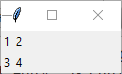
\includegraphics{grid-visa.png}
		\caption{Resultatet av förra slidens kod}
	\end{figure}
	
\end{frame}

\subsection{Place}

\begin{frame}[fragile]
	\frametitle{Placera mera}
	\framesubtitle{Place}
	
	Med \lstinline{place()} placerar man ut elementen på specifika koordinater.
	
	\begin{lstlisting}
app = tk.Tk()
min_widget1 = tk.Label(app, text="1")
min_widget2 = tk.Label(app, text="2")
min_widget3 = tk.Label(app, text="3")
min_widget4 = tk.Label(app, text="4")

min_widget1.place(x=50, y=20)
min_widget2.place(x=20, y=20)
min_widget3.place(x=20, y=50)
min_widget4.place(x=50, y=50)
	\end{lstlisting}

\end{frame}

\begin{frame}
	\frametitle{Placera mera}
	\framesubtitle{Place}
	
	\begin{figure}
		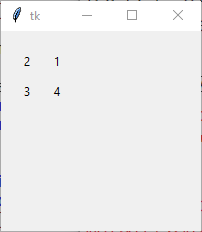
\includegraphics{place-visa.png}
		\caption{Resultatet av förra slidens kod}
	\end{figure}
	
\end{frame}


\section{Knappar}

\begin{frame}[fragile]
	\frametitle{Knappar}
	
	När vi vill lägga till en knapp så skriver vi:
	
	\begin{lstlisting}
import tkinter as tk

def funk():
    ...

root = tk.Tk()

knapp = tk.Button(root, text='Tryck här', command=funk)
	\end{lstlisting}

	Notera att det på rad 8 inte är några paranteser efter funktionsnamnet. Lägg även märke till att funktionen \texttt{funk} inte tar emot några parametrar.

\end{frame}

\begin{frame}[fragile]
	\frametitle{Knappar}
	
	Ett litet exempel
	
	\begin{lstlisting}
import tkinter as tk
def funk():
    tal = fält.get()
    label['text'] = 'Du skrev ' + tal + ' i rutan'
root = tk.Tk()
fält = tk.Entry(root)
label = tk.Label(root)
knapp = tk.Button(root, text='Tryck här', command=funk)
fält.grid(row=1,column=1)
label.grid(row=0, column=1)
knapp.grid(row=1, column=2)
	\end{lstlisting}
	
\end{frame}


\section{Övningar}

\begin{frame}
	\begin{itemize}
		\item Gör ett program som skapar ett fönster
		\item Fönstret ska se ut som följer:
			\begin{center}
				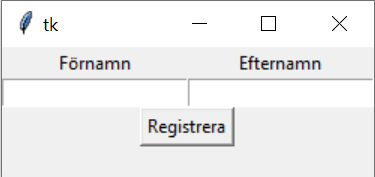
\includegraphics[]{window.png}
			\end{center}		
		\item När man klickar på knappen så ska det understa text-fältet (ett fält under knappen) få texten: ``Namn Namnsson har lagts till''. 
	\end{itemize}
\end{frame}


\end{document}